\chapter{Red Neuronal Convolucional}\label{cnn}

En este capítulo se estudiarán los fundamentos de la red neuronal convolucional (CNN), un subtipo de ANN especializado en el tratamiento de imágenes y usado por aplicaciones actuales de segmentación semántica \ref{apps}.\\

Hasta ahora se ha supuesto que la entrada a una ANN es un vector, algo válido para un gran número de aplicaciones en deep learning. El problema está cuando la entrada de la red neuronal es una imagen. En este caso antes de utilizar la imagen como entrada hay que aplanarla para contener la imagen en un vector, de esta forma cada píxel (px, para imágenes 2D) o vóxel (vx, para imágenes 3D) será un elemento del vector de entrada y estará conectado a cada neurona de la capa siguiente. Para el caso de imágenes pequeñas (como la de la figura \ref{fig:image_to_ANN}) puede ser viable, pero teniendo tan sólo una imagen de $4$x$4$px y 4 neuronas en la única capa oculta, se tendrían $16*4=64$ pesos. Si aplicáramos este sistema a una imagen 3D en escala de grises con $124*124*70=1076320$vx, se necesitarían más de un millón de pesos por cada neurona que haya en la primera capa oculta. Esto hace que sea completamente inviable usar este tipo de redes para imágenes a partir de cierto tamaño. En este capítulo se presentan las redes neuronales convolucionales (CNN), que reducirán en gran medida el nº de pesos necesarios en la red neuronal y aprovecharán técnicas del procesamiento de imágenes para encontrar patrones.

\figura{0.8}{img/image_to_ANN}{Imagen de 4x4 px aplanada y usada como entrada en una FCNN con 4 neuronas en su única capa oculta. No se muestra su capa de salida. Imagen del curso Intro to Deep Learning with PyTorch de Udacity.}{fig:image_to_ANN}{}{Imagen como entrada en una ANN.}

Cambiando la arquitectura de la red vista en la figura \ref{fig:image_to_ANN} por una CNN, obtendríamos una arquitectura similar a la vista en la figura \ref{fig:image_to_CNN}. En esta CNN se ha reducido el nº de conexiones de la capa de entrada a la capa oculta de $64$ a $16$, además, como veremos más adelante, los pesos de las 4 neuronas son compartidos, esto significará que sólo se necesitarán $4$ pesos distintos.

\figura{1}{img/image_to_CNN_}{Imagen de 4x4 px usada como entrada en una CNN. Ambas figuras muestran la misma arquitectura, estando en la figura de la izquierda la imagen aplanada y en la figura de la derecha se muestra la matriz 4x4 como entrada. Imágenes del curso Intro to Deep Learning with PyTorch de Udacity.}{fig:image_to_CNN}{}{Imagen como entrada en una CNN.}

\subsubsection{Conceptos de procesamiento de imagen}

Antes de describir los tipos de capas será necesario introducir varios conceptos propios del procesamiento de imagen que son usados en la capa convolucional (subsección\ref{cnn_capa_conv}) y la capa pooling (subsección \ref{cnn_capa_pooling})

Lo primero es saber que una convolución es una operación matemática entre dos funciones ($f$ y $g$) que produce una tercera función ($f*g$) que expresa cómo la forma de $f$ es cambiada por $g$. \cite{wikipedia_convolution}

En este caso $f$ será la imagen original y $g$ será una matriz con las mismas dimensiones que la imagen. Para facilitar esta explicación se asumirá que la imagen original tiene dos dimensiones, aunque en este proyecto se trabaje con imágenes de tres dimensiones.

Siguiendo este esquema, a $g$ se le conocerá como \textbf{kernel} y definirá la naturaleza de la operación realizada a lo largo de $f$. Si se tiene un kernel $X$ de tamaño $(m,m)$ y una imagen $Y$, esta operación respecto al punto $(y_1, y_2)$ de $Y$ puede definirse cómo la ecuación \ref{eq:kernel}, con un ejemplo visual en la figura \ref{fig:kernel} \cite{convolutionsforimages}

\begin{equation}\label{eq:kernel}
\sum_{k=0}^{m-1}\sum_{l=0}^{m-1} X_{j,k} * Y_{y_1 - i-\lfloor l/2 \rfloor, y_2 -  j -\lfloor l/2 \rfloor}
\end{equation}

\figura{0.4}{img/kernel}{Kernel $2$x$2$ aplicado al elemento $(0,0)$ de una matriz $3$x$3$.}{fig:kernel}{}{Resultado de aplicar un kernel a una imagen.}

En la figura \ref{fig:kernel} se puede observar un problema al intentar aplicar el kernel al punto $(0,2)$. El kernel ``se sale" de la imagen, por lo que no se puede computar esta operación y se pierde información. Para solucionar esto se aplica lo que se conoce como \textbf{padding}.

El padding es una técnica que consiste en añadir píxeles de relleno alrededor de una imagen. En este contexto se añade 0 para evitar alterar los resultados. Un ejemplo de de padding puede verse en la figura \ref{fig:padding} \cite{paddingandstride}.

\figura{0.5}{img/padding}{Kernel $2$x$2$ aplicado al elemento $(0,0)$ de una matriz $3$x$3$ con padding 1 aplicado.}{fig:padding}{}{Resultado de aplicar un kernel a una imagen con padding.}

Esta operación se debe realizar para toda la imagen de entrada. Si se quiere realizar esta operación para todos los puntos de la imagen, el kernel debe ``deslizarse" sobre la imagen elemento a elemento, tanto en horizontal como en vertical. En este caso se dirá que se tiene un \textbf{paso} de 1 horizontal y vertical. En la imagen \ref{fig:paso} \cite{paddingandstride} se puede ver un ejemplo con un paso horizontal de 2 y vertical de 3. De aquí en adelante se supondrá que el paso horizontal y vertical tienen el mismo valor, por lo que el paso estará definido por un solo número.

\figura{0.5}{img/paso}{Kernel $2$x$2$ aplicado a una matriz $3$x$3$ con padding 1, paso horizontal 2 y vertical 3.}{fig:paso}{}{Resultado de aplicar un kernel a una imagen con padding y pasos 2 y 3 para horizontal y vertical.}

Al determinar el kernel, paso y padding se definirá un \textbf{filtro}. Los filtros son de gran interés en el procesamiento de imagen ya que al aplicarlos se pueden producir efectos como desenfoque, realce o detección de bordes. En la figura \ref{fig:filtro} \cite{Wikipedia2020} se muestra un ejemplo de aplicar un filtro a una imagen de entrada.

\begin{figure}[ht]
\centering
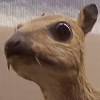
\includegraphics[scale=2]{img/filter_og.png}
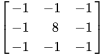
\includegraphics[scale=1]{img/filter_edge_kernel.png}
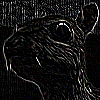
\includegraphics[scale=2]{img/filter_edge.png}
\caption[Resultado de aplicar un filtro de reconocimiento de bordes a una imagen.]{Efecto producido al aplicar un filtro de detección de bordes a una imagen de entrada. La imagen de la izquierda es la imagen de entrada, la central es el kernel y la de la derecha es el resultado final. Imágenes tomadas de la página ``Núcleo (procesamiento digital de imágenes)"\phantom{x} de Wikipedia.}\bigskip
\label{fig:filtro}
\end{figure}

\section{Tipos de capas}\label{cnn_capas}

Antes de describir los tipos de capas usados para construir una  CNN es importante mencionar la \textbf{profundidad}. Cada capa tendrá una profundidad asociada que no hay que confundir con la profundidad de una ANN. En una CNN si una capa tiene profundidad $k$, querrá decir que en esa capa hay un stack de $k$ imágenes en escala de grises. Lo normal es que cada imagen del stack represente características distintas de la imagen de entrada.

A continuación se describirán las capas más comunes usadas en una CNN: Capa Convolucional, Capa de Pooling, Capa ReLU y Capa Completamente Conectada (FC). En la figura \ref{fig:simple-convnet} \cite{missinglink2020} se puede ver un ejemplo en el que la imagen de un barco pasa por varias capas de convolución + ReLU, Pooling y por último FC, dando la predicción de la clase de la imagen.

\figura{1}{img/simple-convnet}{Red Neuronal Convolucional simple en la que la imagen de un barco es clasificada.}{fig:simple-convnet}{}{Ejemplo de CNN en la que se clasifica una imagen con un barco.}

\subsection{Capa convolucional}\label{cnn_capa_conv}

Es la capa principal de este tipo de redes, es donde se aplican los filtros a las imágenes usando convoluciones. Es descrita por 4 hiperparámetros:

\begin{itemize}
\item Número de filtros, \textbf{K}.
\item Tamaño del kernel, \textbf{F}.
\item Paso, \textbf{S}.
\item Padding, \textbf{P}.
\end{itemize}

Esta capa va a tener como entrada una imagen con una profundidad $K_0$, le aplicará un padding de \textbf{P} píxeles/vóxeles alrededor de la imagen y realiza la operación de convolución del stack de imágenes y de $K$ filtros de tamaño $F$ en todas sus dimensiones excepto en la dimensión de la profundidad, que será de tamaño $K_0$. El paso con el que desplazamos los filtros sobre las imágenes será $S$. Suponiendo que la imagen inicial tiene 2D, esta operación se hará frente a una entrada de tamaño $W_1 \times H_1 \times D_1$ y dará como resultado una imagen de tamaño:

\begin{itemize}
\item $W_2 = \frac{W_1 - F}{S} + 1$
\item $H_2 = \frac{H_1 - F}{S} + 1$
\item $D_2 = K$
\end{itemize}

De la misma forma que se han calculado $W$ y $H$ se puede calcular cualquier número de dimensiones. También es importante notar que aunque se puede elegir cualquier valor para $S$, $F$ y $P$, es habitual en las arquitectura modernas que las convoluciones se realicen con $S=1$, $F=3$ y $P=1$, de esta forma quedaría: $W_2 = \frac{W_1-F+2P}{S} + 1 = \frac{W_1 - 3 + 2}{1} + 1 = W_1$. Haciendo esto no varía el tamaño de la imagen.

En la figura \ref{fig:conv-example}\cite{Li2020} se muestra un ejemplo de una capa de convolución de profundidad $2$ con imagen de entrada $5 \times 5$ con $1 px$ de padding y profundidad $3$, siendo los filtros de tamaño $3$ y aplicándose con un paso de $3$. Se obtendrá una imagen $3\times 3$ con profundidad $2$.

Para que la salida tenga profundidad $2$ será necesario usar $2$ filtros. Cada uno de estos filtros tendrá un kernel de tamaño $3\times 3 \times n$, siendo $n=3$ la profundidad de la imagen de entrada a esta capa. Cada kernel tendrá 27 valores, uno por cada píxel. Estos valores son los pesos de las neuronas de la red neuronal y no están definidos por el usuario como los hiperparámetros, en cambio se incializarán de forma aleatoria y se irán modificando acorde al algoritmo de optimización utilizado. Entrenar una CNN significa encontrar unos valores para los filtros que minimicen el error (dado por la función de pérdida). Adicionalmente, también habrá que entrenar la capa FC, que no es más que una red neuronal como ya se ha visto previamente.

\figura{0.8}{img/conv-example}{Capa de convolución de profundidad 2 (se usan dos filtros) con kernel de tamaño $3\times 3 \times 3$ aplicado a una imagen de entrada de tamaño $5\times5$ con profundidad 3 y padding 1. El resultado es un volumen de $3 \times 3 \times 2$.}{fig:conv-example}{}{Ejemplo de capa de convolución.}

\newpage\subsection{Capa Pooling}\label{cnn_capa_pooling}

El objetivo de esta capa es reducir el tamaño de las imágenes para reducir la memoria necesaria y el coste computacional.

De forma similar a la capa de convolución, en la capa de pooling o reducción se usa un filtro que se aplica a toda la imagen. Se diferencian en que esta capa usa un solo filtro de profundidad $1$ que es aplicado a todas las imágenes del stack de entrada, por lo que esta capa mantiene la misma profundidad de la capa anterior. Otra diferencia está en la operación a realizar, en la capa de convolución se aplica un kernel con determinados valores a toda la imagen, en la capa de pooling se usa la función MAX.

Los parámetros necesarios para definir una capa de pooling son:
\begin{itemize}
\item Tamaño del kernel, $F$.
\item Paso, $S$.
\end{itemize} 

Y si se tiene una entrada de tamaño $W_1 \times H_1 \times D_1$, la salida será:
\begin{itemize}
\item $W_2 = \frac{W_1 - F}{S} + 1$
\item $H_2 = \frac{H_1 - F}{S} + 1$
\item $D_2 = D_1$
\end{itemize}

Los parámetros $F$ y $S$ determinan cómo se reducirá la imagen, siendo común usar $F=2$ y $S=2$ para reducir el tamaño a la mitad. Reducir demasiado la imagen al hacer pooling puede provocar un efecto muy destructivo.

\figura{1}{img/maxpool}{Imagen $4\times 4$ a la que se ha aplicado un pooling de $F=2, S=2$. Cada color de la imagen de la izquierda indica las entradas del para la operación MAX, cada color de la imagen de la derecha indica la salida de dicha operación. Figura tomada del curso ``CS231n" de Standford University.}{fig:maxpool}{}{Ejemplo de pooling.}

\subsection{Capa ReLU}\label{cnn_capa_relu}

Esta capa aplica la función de activación no lineal \textit{ReLU} (vista en el apartado \ref{subsubsec:relu}) a cada elemento (píxel o vóxel) de la entrada. Se introduce después de la capa de convolución y es a veces llamada la etapa de detección \cite[335]{Goodfellow2016}.

\subsection{Capa FC}\label{cnn_capa_fc}

Se usa para obtener la puntuación de clase de cada píxel/vóxel de la capa anterior, a la que está completamente conectada (cada nodo de la capa anterior está conectado a todos los de esta capa). Es la salida de la red ya que es la última capa. En problemas de clasificación esta capa tendrá $C$ nodos, siendo $C$ el nº de clases. En problemas de segmentación esta capa tendrá tantos nodos como clases haya multiplicado por el nº píxeles/vóxeles que haya en la capa anterior, entendiéndose la segmentación como etiquetar cada píxel/vóxel con la probabilidad que tiene de pertenecer a cada clase.

Esta capa funciona como una ANN normal, incluyendo los pesos y su actualización.

\section{Funciones de Pérdida}\label{cnn_loss_func}

En esta sección se describirán varias funciones de pérdida que se tuvieron en cuenta en el capítulo \ref{loss_function}, seleccionando finalmente la entropía cruzada binaria.

En las CNNs, al igual que en la inmensa mayoría de algoritmos de deep learning, se usa el descenso por gradiente estocástico o alguna variación como método para optimizar y aprender hacia un objetivo. En este proyecto el objetivo viene dado por la segmentación perfecta realizada de forma manual a la que se llamará $y$. Esta segmentación perfecta se comparará con la predicción obtenida ($\hat{y}$) por el modelo CNN al tomar como dato de entrada la imagen original sin procesar. Como se vio en la sección del descenso por gradiente (\ref{sec:gradient_descent}), se usará una función que tome como entrada la segmentación perfecta y la predicción y devuelva un valor numérico indicando cuánto se aleja la predicción del objetivo. Esta función será la función de pérdida. A continuación se describirán varias funciones de pérdida en relación con el problema de segmentación semántica.

\subsection{Binary Cross-Entropy}\label{cnn_bce}

La entropía cruzada binaria es una medida utilizada para calcular la diferencia entre dos distribuciones de probabilidad. \cite{Jadon2020}. Resultará útil si comparamos el objetivo $y$ con la predicción $\hat{y}$. La fórmula de la entropía cruzada binaria (BCE) es la siguiente:
\begin{equation}
L_{BCE}(y,\hat{y})=-(y log(\hat{y}) + (1-y)log(1-\hat{y}))
\end{equation}

\subsection{Weighted Binary Cross-Entropy}\label{cnn_wbce}

La entropía cruzada binaria con pesos (WCE) es una variante de BCE. En esta variante se aplica un coeficiente a cada ejemplo positivo. Es muy útil cuando los datos están sesgados, como por ejemplo una segmentación de un elemento muy pequeño en comparación con el fondo. La formula es la siguiente:
\begin{equation}
L_{WBCE}(y,\hat{y})=-(\beta y log(\hat{y}) + (1-y)log(1-\hat{y}))
\end{equation}

Para reducir el número de falsos negativos usar $\beta > 1$, para reducir el número de falsos positivos usar $\beta < 1$ \cite{Jadon2020}.

\subsection{Dice Loss}\label{cnn_dice}

El coeficiente Dice se usa como métrica para calcular la similitud entre dos imágenes. En 2016 se adaptó para usarlo como función de pérdida \cite{Cardoso2017}. La fórmula es la siguiente:
\begin{equation}
DL(y,\hat{p})= 1 - \frac{2y\hat{p}+1}{y+\hat{p}+1}
\end{equation}

Siendo $\hat{p}\epsilon[0,1]$ la probabilidad de que un píxel/vóxel pertenezca a una clase, dada por la predicción del modelo, siendo la suma de todas todas las probabilidades (para un determinado píxel/vóxel) igual a $1$.

Se le añade $1$ en el numerador y denominador para evitar que haya $0$ en el numerador o denominador.

